\documentclass[10pt,a4paper]{article}
\usepackage[utf8]{inputenc}
\usepackage[T1]{fontenc}
\usepackage{amsmath}
\usepackage{amsfonts}
\usepackage{amssymb}
\usepackage{graphicx}
\usepackage{listings}
\usepackage{float}
\usepackage{multirow}
\usepackage{subcaption}
\usepackage[table]{xcolor}
\usepackage[labelformat=parens,labelsep=quad,skip=3pt]{caption}


\begin{document}
	\title{Homework 4 - Resource Handling}
	\makeatletter
	
	\author{Zackary McClamma\thanks{University of Dayton}
		\thanks{Dept. of Electrical and Computer
			Engineering, University of Dayton, 300 College Park, Dayton, OH
			45469-0226, U.S.A. E-mail:
			mcclammaz1@udayton.edu}}
	
	\makeatother
	
	\date{\today}
	
	\maketitle
	\section{Introduction}
	This homework assignment was focused on resource sharing and consisted of running the $\mu$C/OS-II\texttrademark operating system with two tasks, a mutex, and custom UART print function. Each task prints the alphabet, one in lowercase and the other in uppercase. The basic idea is that if the tasks have short enough delays after the print statements they will interfere with one another and cause the output to become jumbled. Adding the mutex fixes this issue as it locks the print resource down while a task is printing and the other task has to wait for the resource, in this case the UART port.
	
	\section{System Design}
 	This is a fairly simple system the only peripheral is the UART port and a clock. The operating system does most of the work without much input. The UART port is used to connect the device to an external computer where a terminal can be opened to monitor the output of the development board. Writing to this port can be accomplished with the standard printf fucntion, but, in this case to have more control over the resource a custom UART print function, which will be explained in the section 3 of this document, was created.

	
	\section{Theory of Operation}
	In this system the majority of the work is done in software since the only peripherals are the UART connection and  a clock. The Nios-II processor is first loaded onto the FPGA along with the memory. The operating system is then loaded onto the processor and is used to create two tasks. The first task prints a lowercase alphabet and the second an uppercase alphabet. Initially the program was run with no mutex and the tasks were set to have a difference between delays of 5ms to check that the print statements did in fact interfere with one another. After that was tested the mutex was added to lock the resources when in use which should allow for the print statement to be executed without interference. The uartPrint function is another crucial part of this program not shown in the diagram explicitly, it polls the UART register, checking the transmit status bit if the bit is a 1 then the register is available, if it is a 0 the function continues polling. Once the status bit is read as a 1 the function then writes a byte to the transmit data part of the register and then goes back to polling for the status bit until it is available and can write the next byte. This continues until the string reaches a null character since that is how C terminates strings. 
	\begin{figure}[H]
		\centering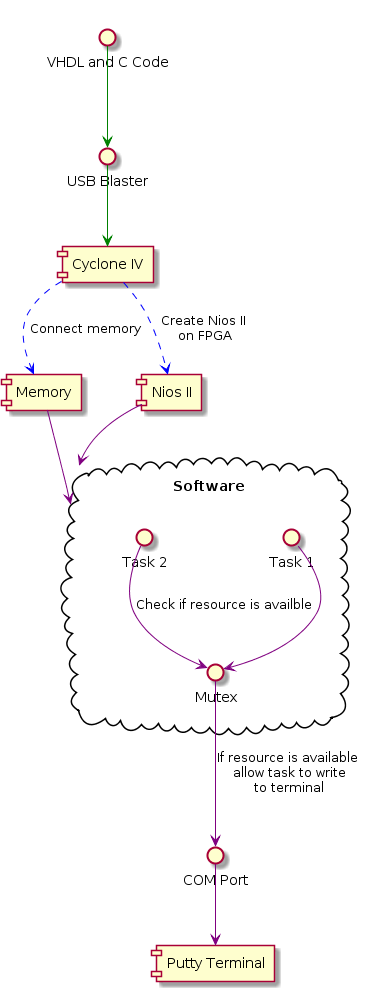
\includegraphics[height=15cm]{HW4_Block.png}
		\caption{Embedded System Block Diagram}
		\label{block}
	\end{figure}


	\section{Results}
	In the screenshots below Figure \ref{notex} demonstrates how the program functions without a mutex. As can be seen in the screenshot the print statements are clearly interfering with one another because there are capital letters being printed with lower case letters. Figure \ref{tex} shows the results when the mutex is added, and as can clearly be seen the mutex prevents the print statements from interfering with one another.
	\begin{figure}[H]
	\centering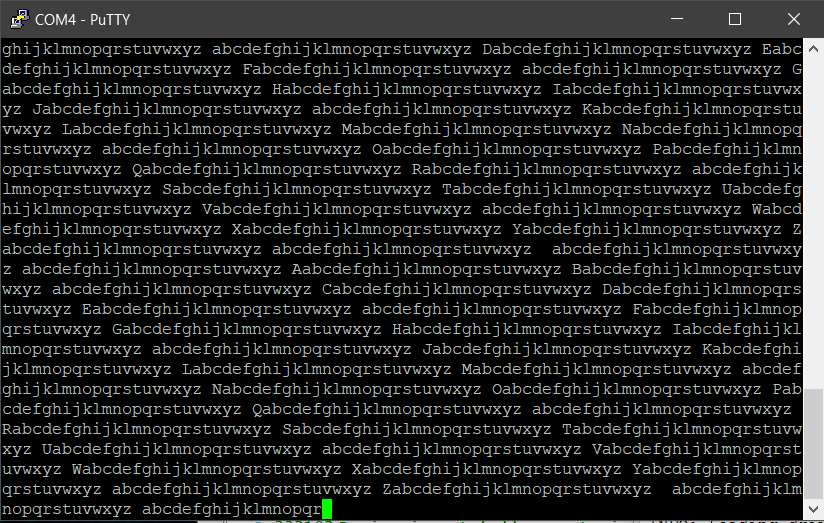
\includegraphics[width=15cm]{Output_No_Mutex.png}
	\caption{Terminal output without Mutex}
	\label{notex}
	\end{figure}
	\begin{figure}[H]
		\centering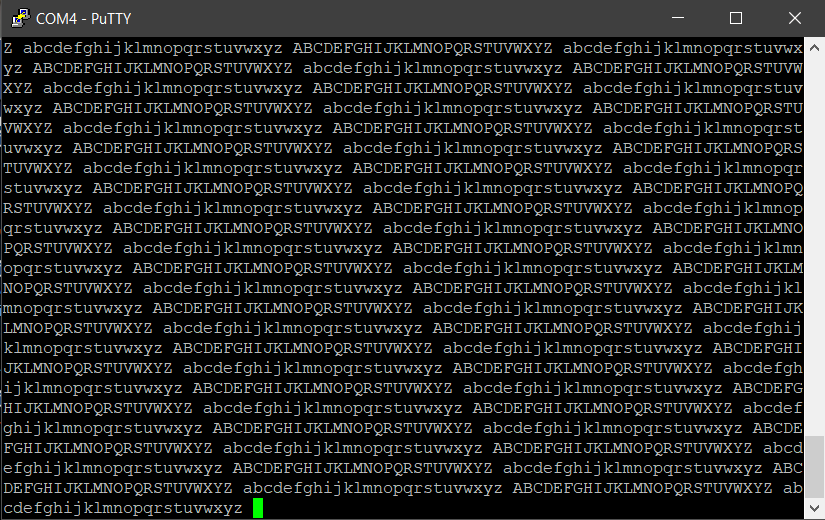
\includegraphics[width=15cm]{Output_With_Mutex.png}
		\caption{Terminal output with Mutex}
		\label{tex}
	\end{figure}

	\section{Conclusion}
	Overall this was a fairly simple assignement, I have already worked with mutexes and semaphores in the past so I was farmilar with them. The only difficult part about this project was getting the print function right and the only reason I got hung up on it was because I made a small logic error that I didn't notice until I had already ran the program about 100 times. The problem I had was that I was using the while loop that polls the status register as an if statement instead of a while loop so I was checking if the bit was 1 not 0 which caused my program to reach the polling loop and stall there because nothing was ever written to the transmit register the value was always 1.
	\clearpage
	\appendix
	\section{\\VHDL Code}
	\lstinputlisting[language=VHDL]{homework4.vhd}
	
	\section{\\C Code}
	\subsection{Headers}
	\lstinputlisting[language=C]{hw4.h}
	
	\subsection{Source}
	\lstinputlisting[language=C]{main.c}
\end{document}